\chapter{Architecture technique et conception des modules}
\label{chap:architecture}

\section{Introduction}

Après avoir défini les besoins du système et préparé les données, il est désormais essentiel d'aborder l'\textbf{aspect technique} du projet. Ce chapitre a pour objectif de présenter l'architecture globale d'AutoMaze AI, en détaillant le rôle de chaque module ainsi que leurs interactions. Une attention particulière sera accordée à la \textbf{séparation entre la vérité terrain du simulateur et la perception du modèle}, qui garantit que les décisions du véhicule reflètent réellement la qualité de notre classifieur.

\section{Architecture globale d'AutoMaze AI}

L'architecture du projet repose sur un principe simple. Le simulateur connaît la position de chaque objet présent dans son environnement, tandis que le \textbf{modèle de Machine Learning} analyse l'image fournie par la caméra virtuelle et en détermine la nature. Le système associe ensuite la classe prédite à la position connue de l'objet. Le \textbf{planificateur} calcule le chemin vers la destination et le recalcule lorsqu'un obstacle rend le trajet impraticable. Enfin, le \textbf{contrôleur} applique les décisions au véhicule virtuel : continuer, ralentir, s'arrêter ou changer de direction.

\begin{figure}[H]
  \centering
  \resizebox{\textwidth}{!}{% Architecture fonctionnelle globale d'AutoMaze AI (cinq étages, de l'environnement au contrôleur)
\begin{tikzpicture}[
    etage/.style={draw=accent, fill=accent!7, rounded corners=3pt, align=center, font=\footnotesize,
                  text width=12.2cm, minimum height=1.0cm, inner sep=4pt},
    bloc/.style={draw=black!60, fill=white, rounded corners=3pt, align=center, font=\footnotesize,
                 text width=3.6cm, minimum height=1.05cm, inner sep=3pt},
    ml/.style={bloc, draw=accent, fill=accent!18, very thick},
    fleche/.style={-{Stealth[length=2.2mm]}, draw=black!70, thick}
  ]
  \node[etage] (env) at (0,0) {\textbf{1. Environnement de simulation}\\Routes · Véhicule · Objets routiers · Destination};

  \node[bloc] (camera) at (-4.3,-1.75) {\textbf{Caméra virtuelle}\\Image de l'objet};
  \node[ml] (modele) at (-4.3,-3.35) {\textbf{Modèle ML}\\Classification de l'objet};
  \node[bloc] (infos) at (4.3,-2.55) {\textbf{Informations du simulateur}\\Coordonnées et positions des objets};
  \node[bloc] (etat) at (0,-4.75) {\textbf{État des obstacles}\\Position + nature identifiée};

  \node[etage] (fusion) at (0,-6.3) {\textbf{2. Fusion des informations et représentation de l'environnement}\\Association de la classe prédite aux coordonnées de l'objet correspondant};
  \node[etage] (plan) at (0,-7.75) {\textbf{3. Planificateur}\\Graphe · Dijkstra · Recalcul du trajet};
  \node[etage] (decision) at (0,-9.2) {\textbf{4. Système de décision}\\Ralentir · Arrêter · Contourner · Continuer};
  \node[etage] (controle) at (0,-10.65) {\textbf{5. Contrôleur du véhicule}\\Vitesse · Freinage · Direction};
  \node[font=\footnotesize\bfseries, text=integration] (but) at (0,-11.75) {Déplacement autonome jusqu'à la destination};

  \draw[fleche] (env.south -| camera) -- (camera);
  \draw[fleche] (camera) -- (modele);
  \draw[fleche] (env.south -| infos) -- (infos);
  \draw[fleche] (modele.south) |- (etat.west);
  \draw[fleche] (infos.south) |- (etat.east);
  \draw[fleche] (etat) -- (fusion);
  \draw[fleche] (fusion) -- (plan);
  \draw[fleche] (plan) -- (decision);
  \draw[fleche] (decision) -- (controle);
  \draw[fleche] (controle) -- (but);

  % Une décision qui bloque un tronçon relance le planificateur
  \draw[fleche, dashed, draw=accent] (decision.east) -- ++(0.55,0) |- node[pos=0.25, right, font=\scriptsize, align=left, text=accent] {obstacle\\bloquant :\\recalcul} (plan.east);
  % Le véhicule se déplace dans l'environnement : la boucle reprend
  \draw[fleche, draw=integration] (but.west) -- ++(-6.9,0) |- node[pos=0.25, left, font=\scriptsize, text=integration, align=right] {nouvelle\\position} (env.west);

  % Ce que le simulateur ne transmet pas
  \node[font=\scriptsize, text=black!65, align=center, text width=3.8cm] at (4.3,-3.95) {La vraie classe de l'objet n'est jamais transmise à la décision};
\end{tikzpicture}
}
  \caption{Architecture fonctionnelle globale d'AutoMaze AI}
  \label{fig:architecture}
\end{figure}

\section{Environnement de simulation}
\label{sec:environnement}

Notre environnement de simulation reproduit une partie réelle de \textbf{Casablanca}, du Twin Center (Maârif) à la place Mohammed V. Le réseau routier provient d'\textbf{OpenStreetMap} et respecte les sens uniques. Le véhicule circule à 8~m/s, soit environ 29~km/h, et le temps avance par pas d'une seconde. Chaque épisode place six obstacles sur l'itinéraire, et trois vues sont proposées : une carte en 2D, une vue conducteur et une vue en 3D.

Les simulateurs de conduite professionnels offrent des environnements 3D très détaillés, comme l'illustre la figure~\ref{fig:inspiration}. Notre simulateur reste volontairement plus simple, puisqu'il sert uniquement à démontrer l'utilisation du modèle.

\begin{figure}[H]
  \centering
  \begin{subfigure}[t]{0.49\textwidth}
    \centering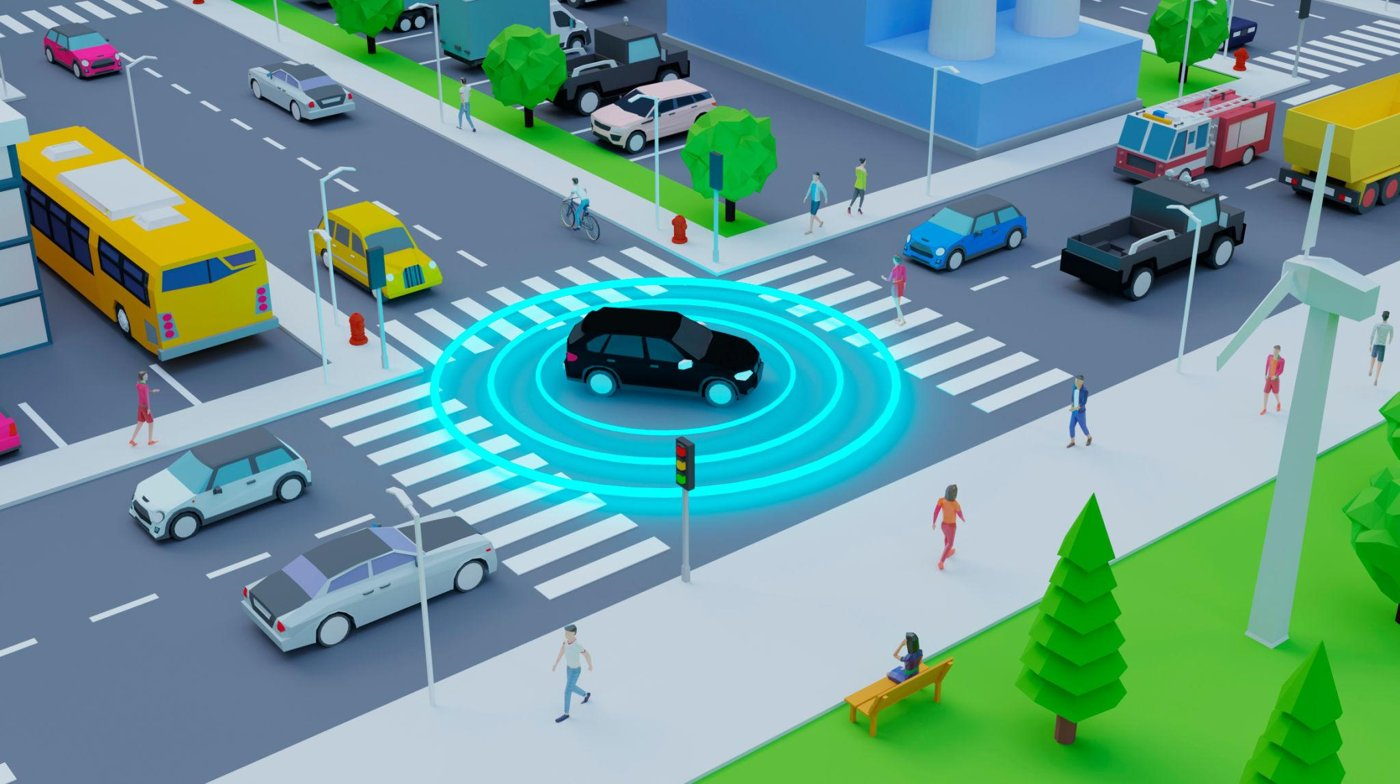
\includegraphics[width=\textwidth]{environnement_vir1.jpg}
  \end{subfigure}\hfill
  \begin{subfigure}[t]{0.49\textwidth}
    \centering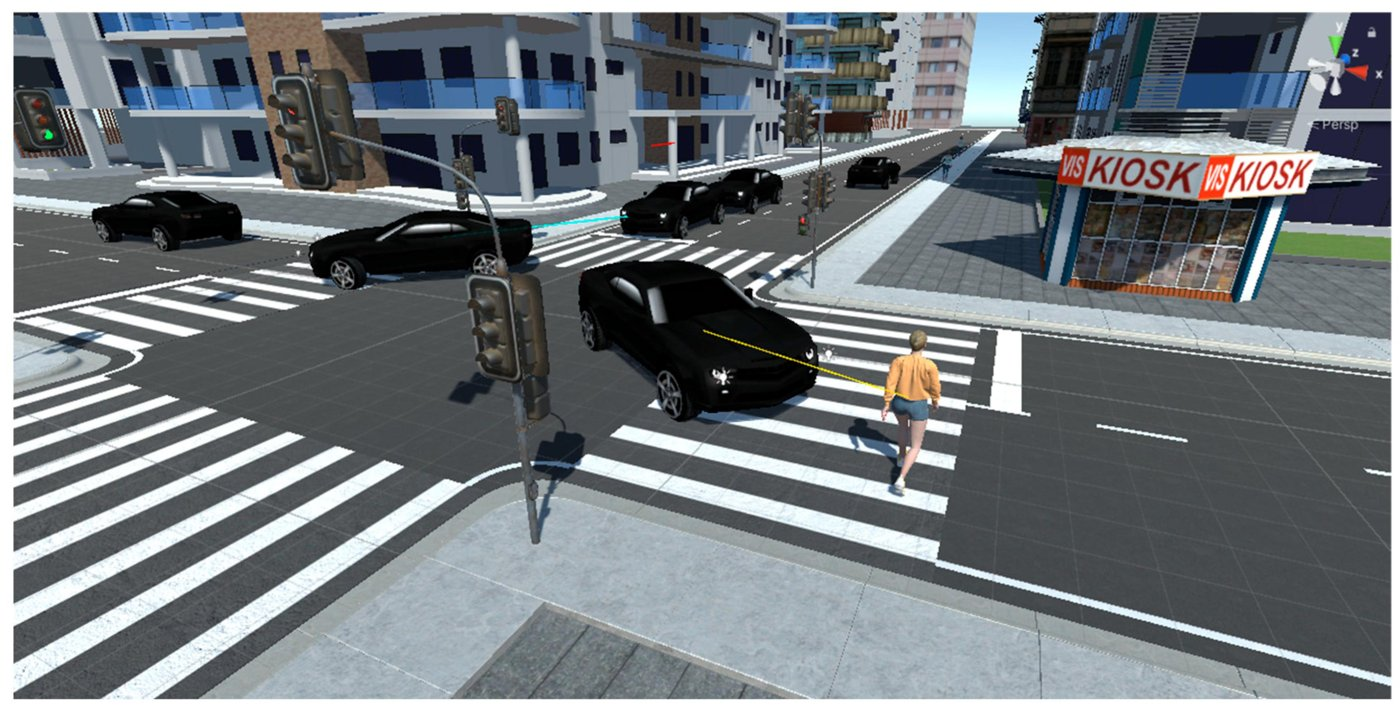
\includegraphics[width=\textwidth]{environnement_vir2.jpg}
  \end{subfigure}
  \caption{Exemples d'environnements virtuels de conduite ayant servi d'inspiration (sources externes)}
  \label{fig:inspiration}
\end{figure}

\begin{figure}[H]
  \centering
  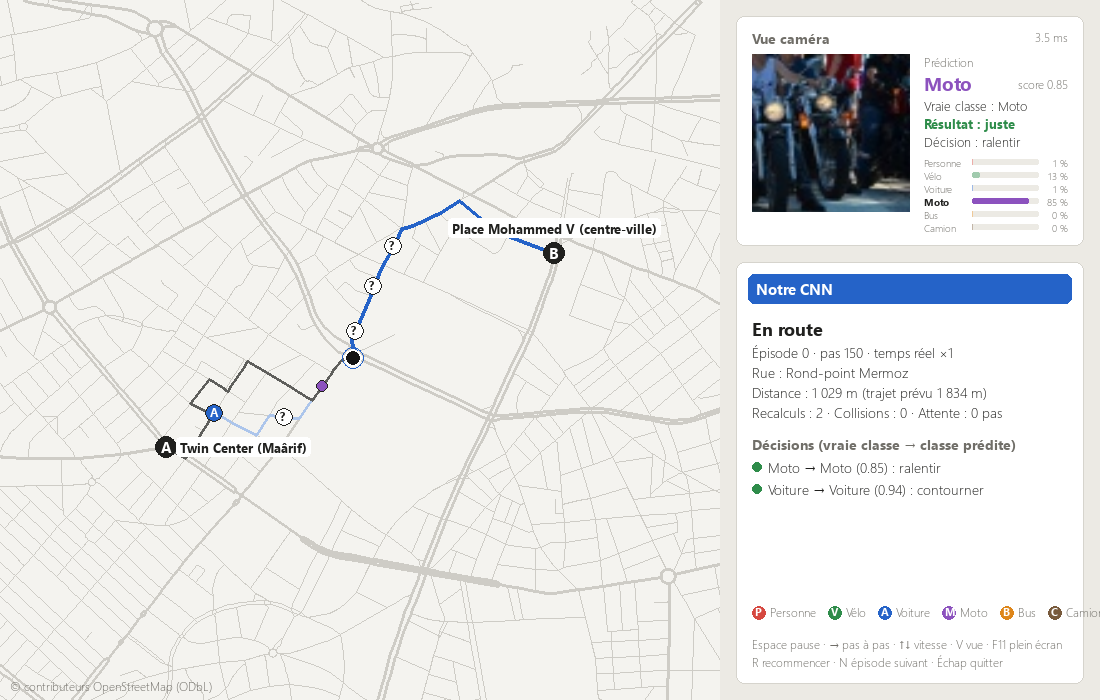
\includegraphics[width=0.82\textwidth]{06_simulateur_carte.png}
  \caption{Notre simulateur en vue carte : itinéraire, obstacles et dernière prédiction (carte © contributeurs OpenStreetMap)}
  \label{fig:notre-simulateur}
\end{figure}

\section{Acquisition des images par caméra virtuelle}
\label{sec:camera}

Lorsqu'un obstacle se trouve sur l'itinéraire à moins de 35~m, la \textbf{caméra virtuelle} transmet son image au modèle.

Ce module repose sur un choix de conception important. Si la caméra filmait les objets 3D du simulateur, le modèle recevrait des images de synthèse très différentes des photos sur lesquelles il a appris, et ses performances chuteraient. La caméra fournit donc une \textbf{vraie photo} de la classe de l'obstacle, tirée du jeu de test, que le modèle n'a jamais vue. Les modèles 3D servent uniquement à l'affichage. De plus, une même graine aléatoire donne les mêmes images à tous les classifieurs comparés, tandis que les images changent d'un épisode à l'autre.

\subsection{Association d'une image à chaque objet}

L'association entre un objet du simulateur et l'image transmise au modèle se déroule en quatre étapes :

\begin{enumerate}
  \item \textbf{Création de l'obstacle}\\
  Au début de chaque épisode, le simulateur place six obstacles sur l'itinéraire. Chacun reçoit une position (un tronçon de rue et une distance sur ce tronçon) ainsi qu'une vraie classe, tirée au hasard parmi les six.
  \item \textbf{Choix de l'image}\\
  Lorsque le véhicule arrive à moins de 35~m de l'obstacle, la caméra virtuelle choisit une image dans le dossier du jeu de test correspondant à sa vraie classe (\texttt{data/crops/test/<classe>/}). Si l'obstacle est un camion, la caméra \og voit \fg{} donc la photo d'un vrai camion que le modèle n'a jamais rencontrée.
  \item \textbf{Tirage reproductible}\\
  Le choix de l'image dépend de la graine de l'expérience, de la position de l'obstacle et du numéro de l'épisode. Ainsi, un même obstacle reçoit toujours la même image, quel que soit le classifieur testé, ce qui garantit une comparaison équitable. L'image est ensuite conservée en mémoire, afin que le véhicule voie la même photo s'il repasse devant l'obstacle.
  \item \textbf{Transmission au modèle}\\
  L'image est transmise au classifieur actif, sans aucune indication sur sa vraie classe. La prédiction obtenue est alors rattachée à l'obstacle d'origine (section~\ref{sec:association}).
\end{enumerate}

La vraie classe sert donc uniquement à choisir ce que la caméra \og voit \fg{}, comme dans la réalité, où un camion présent sur la route apparaît sur l'image de la caméra. Elle n'intervient jamais dans la décision du véhicule, qui repose seulement sur la prédiction du modèle. Si aucune image n'est disponible pour une classe, par exemple avant la préparation des données, le simulateur génère une image de remplacement.

\section{Module de classification par Machine Learning}
\label{sec:module-classification}

Le module de classification reçoit l'image RGB d'un objet, quelle que soit sa taille, et applique lui-même le prétraitement : mise au carré, réduction à 64~×~64~px et normalisation. Il renvoie ensuite :

\begin{itemize}
  \item la \textbf{classe prédite}, parmi les six classes ;
  \item un \textbf{score de confiance}, correspondant au plus grand des six scores ;
  \item les \textbf{six scores}, dont la somme vaut 1 ;
  \item le \textbf{temps de calcul} réellement mesuré.
\end{itemize}

L'affichage prend par exemple la forme \og Image \textrightarrow{} Voiture (92~\%) \fg{}. Ce pourcentage est un exemple d'affichage et non une performance mesurée. Il s'agit d'un score et non d'une probabilité calibrée, ce qui signifie que le modèle n'a pas forcément raison 92 fois sur 100.

Lorsque le score est inférieur à un certain seuil, la classe devient \og Inconnu \fg{} et le véhicule effectue un arrêt prudent. Ce \textbf{seuil} sera choisi sur le jeu de validation, puis enregistré avec le modèle.

Enfin, trois classifieurs respectent la même interface et sont donc interchangeables : un mode \og simulation \fg{}, qui permet de tester la logique sans modèle, notre propre modèle, et un éventuel modèle de référence préentraîné, utilisé uniquement comme point de comparaison si l'encadrante l'accepte.

\section{Module de localisation et association des objets}
\label{sec:association}

Le simulateur décrit chaque obstacle par un identifiant et une position sur la carte, comme le montre l'exemple suivant.

\begin{table}[H]
\centering
\small
\caption{Exemple d'association entre position et classe prédite}
\begin{tabularx}{\textwidth}{>{\raggedright\arraybackslash}p{2cm}>{\raggedright\arraybackslash}p{4.4cm}>{\raggedright\arraybackslash}p{2.6cm}Y}
  \toprule
  \entete \textbf{Identifiant} & \textbf{Position} & \textbf{Classe prédite} & \textbf{Vraie classe (cachée)} \\
  \midrule
  OBJ-01 & Tronçon A \textrightarrow{} B, à 45~m de A & Voiture & Voiture \\
  OBJ-02 & Tronçon C \textrightarrow{} D, à 12~m de C & Personne & Personne \\
  OBJ-03 & Tronçon E \textrightarrow{} F, à 30~m de E & Voiture & Camion \\
  \bottomrule
\end{tabularx}
\end{table}

L'\textbf{association} entre une prédiction et un objet est directe : chaque image est produite pour un obstacle précis, et la prédiction est donc rattachée à l'objet dont elle provient. Ce choix, simple et sûr, est possible car chaque image ne contient qu'un seul objet.

Il est essentiel de bien séparer deux types d'informations :

\begin{itemize}
  \item \textbf{La vérité terrain}\\
  Elle regroupe la vraie classe et la position de l'objet. Elle sert à construire les scénarios, à faire agir l'obstacle selon sa vraie nature (une personne finit de traverser, un camion reste immobile) et à mesurer les erreurs.
  \item \textbf{La perception}\\
  Elle correspond à la classe prédite par notre modèle. C'est la seule information transmise au système de décision. Une erreur du modèle a donc de vraies conséquences, comme dans le cas de l'objet OBJ-03, qui peut mener à une collision.
\end{itemize}

\section{Représentation de l'environnement et des obstacles}

L'environnement est représenté sous forme de \textbf{graphe orienté}, dont les nœuds sont les intersections et les arêtes les tronçons de rue. Chaque tronçon possède un coût égal à sa longueur en mètres, éventuellement multipliée par une pénalité. Un obstacle peut modifier ce graphe de trois manières :

\begin{itemize}
  \item en \textbf{bloquant} un tronçon, définitivement ou pendant quelques pas ;
  \item en \textbf{pénalisant} un tronçon, c'est-à-dire en multipliant son coût ;
  \item en pénalisant également les \textbf{tronçons voisins}, dans le cas d'un gros véhicule.
\end{itemize}

\section{Algorithme de planification Dijkstra}

L'algorithme de \textbf{Dijkstra}, implémenté directement dans le projet plutôt qu'emprunté à une bibliothèque, calcule le chemin de coût minimal entre la position actuelle du véhicule et sa destination. Après chaque modification du graphe, il est relancé depuis la position du véhicule. Si l'obstacle se trouve sur le tronçon actuel, le véhicule peut faire demi-tour, et les sens uniques sont toujours respectés.

Il faut toutefois noter que le chemin le plus court n'est pas toujours le plus rapide ni le plus sûr. Nous utilisons donc les distances comme coûts de départ, puis nous ajoutons des pénalités pour les passages moins favorables, par exemple une rue où circule un vélo.

\subsection{Justification du choix de Dijkstra}

Le choix de Dijkstra répond d'abord à un \textbf{objectif pédagogique} : il s'agit de mettre en pratique, dans un cas concret, l'un des algorithmes de graphes étudiés en première année. La planification n'étant pas le cœur scientifique du projet, nous avons privilégié un algorithme que l'équipe maîtrise et peut expliquer en détail, plutôt qu'une méthode plus avancée.

Ce choix reste par ailleurs \textbf{adapté au problème}, pour plusieurs raisons :

\begin{itemize}
  \item \textbf{Des coûts toujours positifs}\\
  Les coûts sont des longueurs en mètres, éventuellement multipliées par une pénalité supérieure à 1. Ils sont donc toujours positifs, ce qui est la condition pour que Dijkstra trouve le plus court chemin exact.
  \item \textbf{Un graphe de taille modeste}\\
  La zone simulée compte 1~387 intersections et 2~907 tronçons de rue. Avec une file de priorité, Dijkstra calcule l'itinéraire de 1~834~m entre le Twin Center et la place Mohammed V en 5~ms environ sur un processeur ordinaire, ce qui permet de le relancer après chaque obstacle.
  \item \textbf{Un résultat exact et facile à vérifier}\\
  L'algorithme ne repose sur aucune approximation, ce qui facilite l'écriture de tests automatiques sur de petits graphes dont la solution est connue.
\end{itemize}

\begin{table}[H]
\centering
\small
\caption{Comparaison des algorithmes de plus court chemin envisagés}
\begin{tabularx}{\textwidth}{>{\raggedright\arraybackslash}p{3.2cm}YY}
  \toprule
  \entete \textbf{Algorithme} & \textbf{Intérêt} & \textbf{Limite pour notre projet} \\
  \midrule
  \textbf{Dijkstra (retenu)} & Chemin le plus court exact avec des coûts positifs, algorithme étudié en première année & Explore plus de nœuds que A*, ce qui reste sans conséquence sur un graphe de cette taille \\
  Parcours en largeur (BFS) & Très simple & Ne tient pas compte des longueurs des rues, seulement du nombre de tronçons \\
  A* & Plus rapide sur de très grands graphes grâce à une estimation de la distance restante & Gain inutile ici, et une heuristique supplémentaire à justifier \\
  Bellman-Ford & Accepte des coûts négatifs & Plus lent, alors que nos coûts sont toujours positifs \\
  \bottomrule
\end{tabularx}
\end{table}

\section{Système de décision}

Le système de décision traduit les informations de perception et de planification en actions. Une décision n'est déclenchée que pour un obstacle situé sur l'itinéraire, devant le véhicule et à moins de 35~m.

\begin{table}[H]
\centering
\small
\caption{Règles de décision selon la situation rencontrée}
\begin{tabularx}{\textwidth}{>{\raggedright\arraybackslash}p{3.4cm}>{\raggedright\arraybackslash}p{3.2cm}Y}
  \toprule
  \entete \textbf{Situation} & \textbf{Décision} & \textbf{Effet} \\
  \midrule
  Aucun obstacle sur la trajectoire & Continuer & Le véhicule suit son itinéraire \\
  Personne & S'arrêter et attendre & Attente de 5 pas, puis reprise du même trajet \\
  Vélo ou moto & Ralentir & Tronçon 3 fois plus coûteux, vitesse divisée par 3 s'il reste le meilleur chemin \\
  Voiture & Contourner & Tronçon bloqué, puis nouvel itinéraire \\
  Bus ou camion & Contourner largement & Tronçon bloqué, rues voisines 10 fois plus coûteuses, puis nouvel itinéraire \\
  Score trop faible (\og Inconnu \fg{}) & Arrêt prudent & Attente de 2 pas, tronçon bloqué, puis nouvel itinéraire \\
  Aucun chemin possible & Rester arrêté & Nouvel essai à chaque pas, épisode \og bloqué \fg{} après 30 pas \\
  Voie dégagée (fin de l'attente) & Reprendre & Le véhicule repart sur son itinéraire \\
  \bottomrule
\end{tabularx}
\end{table}

Dans cette première version, l'action dépend uniquement de la classe prédite, la distance et la position de l'objet servant seulement à déclencher la décision. Une règle plus réaliste devrait également tenir compte de la distance, de la trajectoire et de la vitesse relative. En effet, un piéton sur le trottoir ne demande pas le même arrêt qu'un piéton sur la chaussée. Ce raffinement pourra être ajouté si le temps le permet.

\section{Contrôle du véhicule virtuel}

Le contrôleur reçoit les actions décidées et commande le véhicule virtuel. Il reste volontairement simplifié et ne modélise ni les forces ni l'adhérence. À chaque pas, il applique l'une des commandes suivantes :

\begin{itemize}
  \item \textbf{avancer} de 8~m le long de l'itinéraire ;
  \item \textbf{ralentir}, en divisant la vitesse par 3 sur un tronçon pénalisé ;
  \item \textbf{s'arrêter} pendant le nombre de pas décidé ;
  \item \textbf{changer de direction} en suivant le nouvel itinéraire, ou faire demi-tour si nécessaire ;
  \item \textbf{reprendre} le déplacement lorsque la voie est libre.
\end{itemize}

Une collision est comptée lorsque le véhicule atteint un obstacle encore présent. Cette situation peut se produire, par exemple, si un camion immobile a été confondu avec un vélo : le véhicule ralentit alors au lieu de contourner.

\section{Communication et intégration des modules}

La communication entre les modules repose sur quelques points d'échange bien définis, qui limitent les risques d'incompatibilité.

\begin{table}[H]
\centering
\small
\caption{Points d'échange entre les modules}
\begin{tabularx}{\textwidth}{>{\raggedright\arraybackslash}p{4.2cm}Y}
  \toprule
  \entete \textbf{Point d'échange} & \textbf{Rôle} \\
  \midrule
  \texttt{simulator/contracts.py} & Seul fichier partagé entre les modules, il définit la prédiction, l'obstacle, les actions et l'interface commune des classifieurs \\
  \texttt{models/metadata.json} & Décrit le modèle : ordre des classes, taille d'entrée, ordre des couleurs, normalisation et seuil \\
  Poids du modèle & Chargés par le simulateur, qui ne réentraîne jamais le modèle \\
  Journal des rencontres & Une ligne par obstacle (vraie classe, classe prédite, score, action, temps), utilisée pour mesurer les erreurs \\
  \bottomrule
\end{tabularx}
\end{table}

Au chargement du modèle, le simulateur vérifie que l'ordre des classes est correct, car une inversion transformerait par exemple un bus en personne sans aucun message d'erreur. Un test de concordance compare également les sorties du simulateur et celles du notebook sur les mêmes images, afin de garantir que le prétraitement est identique.

\section{Conclusion}

Ce chapitre a permis de présenter l'\textbf{architecture technique d'AutoMaze AI} et le fonctionnement détaillé de chacun de ses modules. L'approche retenue garantit une séparation claire entre la vérité terrain du simulateur et la perception du modèle, ce qui permet de mesurer réellement l'apport de la classification. Les choix effectués pour la caméra virtuelle, l'association des objets, la planification et la décision assurent la cohérence de l'ensemble. Le chapitre suivant présente la méthodologie expérimentale qui permettra d'entraîner et d'évaluer les classifieurs.
